\documentclass[9pt,twocolumn,twoside,lineno]{gsag3jnl}
\usepackage{epstopdf}
\usepackage{graphicx}
\usepackage{booktabs}
\usepackage{amsmath}
\usepackage{url}

\articletype{inv}

\runningtitle{Attention Pooling for GPT-2 Sentiment Analysis}

\runningauthor{Saleh, Hany, and Khamis}

\title{Improving GPT-2 Sentiment Classification via Learned Attention Pooling}

\author[$\ast$,1]{Ahmed Saleh}
\author[1]{Mohamed Hany}
\author[1]{Mostafa Khamis}

\affil[1]{AIU -- AIE241}

\correspondingauthoraffiliation[$\ast$]{Corresponding author: a.saleh.dev@gmail.com}

\begin{abstract}
Fine-tuning pre-trained language models for downstream classification tasks typically uses the hidden state of the final token as the sentence representation. While effective for many tasks, this approach may be suboptimal for long documents where sentiment-relevant information is distributed across the text. We propose \textbf{gated attention pooling}, which replaces the standard softmax-based attention with independent sigmoid gates, removing the unwanted competition between tokens imposed by softmax normalization. We evaluate our method on two sentiment analysis datasets: SST (5-class, short sentences) and CFIMDB (binary, long reviews), under both frozen and fine-tuning regimes. On CFIMDB with a frozen GPT-2 encoder, gated attention pooling improves accuracy from 88.57\% to 95.10\% (+7.33\%), outperforming standard softmax attention pooling (93.88\%) by 1.22\%. Our method adds only 769 parameters and requires no changes to the underlying language model.
\end{abstract}

\keywords{Sentiment Analysis; GPT-2; Attention Pooling; Transfer Learning}

\begin{document}

\maketitle
\thispagestyle{firststyle}
\firstpagefootnote
\vspace{-13pt}

\section{Introduction}

Large pre-trained language models such as GPT-2~\citep{radford2019language} and BERT~\citep{devlin2019bert} have become the foundation for modern natural language processing. The dominant paradigm is to pre-train on a large corpus, then fine-tune on a downstream task. For sentence-level classification tasks, a common approach is to take the final hidden state of a designated token (the [CLS] token in BERT, or the last token in causal LMs like GPT-2) and pass it through a linear classifier.

This last-token pooling strategy works well for short texts where the final token can attend to the entire sequence. However, for longer documents---such as movie reviews averaging 192 words---sentiment-relevant information may be distributed across the text, and the final token may not capture the most informative signals. Uniform mean pooling is a natural alternative but can dilute strong sentiment signals by averaging with neutral filler tokens.

We propose \textbf{attention pooling}: a learned weighted average of all token hidden states, where the model learns to assign higher weight to sentiment-bearing tokens. This adds a minimal number of parameters (769 for GPT-2's 768-dimensional hidden states) and can be applied without modifying the underlying language model.

Our contributions are:
\begin{itemize}
\item We identify a limitation of last-token pooling for long-document sentiment analysis with frozen encoders.
\item We introduce \textbf{gated attention pooling}, which replaces softmax with independent sigmoid gates, removing the unwanted competition between tokens imposed by the softmax normalization.
\item We demonstrate a +7.33\% improvement over baseline on CFIMDB frozen (88.57\% to 95.10\%), and a +1.22\% improvement over standard softmax attention pooling (93.88\% to 95.10\%).
\item We provide ablation comparing last-token, mean, softmax attention, and gated attention pooling across multiple settings.
\end{itemize}

\section{Related Work}

\textbf{Sentiment Analysis with Pre-trained LMs.} The AIE241 Default Project~\citep{cs224n2024} provides a standard baseline for sentiment analysis using GPT-2 with last-token pooling, establishing reference accuracies for both SST and CFIMDB datasets. Our work builds directly on this baseline.

\textbf{Pooling Strategies for Sequence Classification.} The standard approach in BERT-style models is to use the [CLS] token's hidden state~\citep{devlin2019bert}. For causal LMs like GPT-2, the last token is typically used since it has attended to all previous positions~\citep{radford2019language}. Lin et al.~\citep{lin2017structured} proposed self-attentive sentence embeddings that learn to extract multiple aspects of a sentence. Our work is simpler---a single learned attention head---and focuses specifically on the frozen LM setting where the encoder weights cannot be adapted.

\textbf{Gradient Accumulation and Memory Constraints.} When fine-tuning large models on consumer GPUs, gradient accumulation is essential to simulate larger batch sizes without exceeding GPU memory~\citep{radford2019language}. Our experiments on CFIMDB use accumulation factor 2 to compensate for reduced batch size.

\section{Methods}

\subsection{Datasets}

We evaluate on two datasets from the AIE241 Default Project~\citep{cs224n2024}:

\textbf{SST (Stanford Sentiment Treebank)}~\citep{socher2013recursive} consists of movie review sentences with 5-class sentiment labels (very negative to very positive). Sentences average 19 words in length. The dataset is split into 8,544 train, 1,101 dev, and 2,210 test examples.

\textbf{CFIMDB} is a binary sentiment classification dataset derived from the Large Movie Review Dataset~\citep{maas2011learning}, using the CS224N subset: 1,701 train, 245 dev, and 488 test examples. Reviews average 191 words, making this the primary test case for our hypothesis that last-token pooling is suboptimal for long documents.

\subsection{Model Architecture}

We use GPT-2-small (124M parameters) as our base encoder. For each input sequence, GPT-2 produces a sequence of hidden states $\mathbf{H} = [\mathbf{h}_1, \mathbf{h}_2, \ldots, \mathbf{h}_n]$ where $\mathbf{h}_i \in \mathbb{R}^{768}$.

\textbf{Baseline: Last-Token Pooling.} The sentence representation is the hidden state of the final non-padding token:
\begin{equation}
\mathbf{s} = \mathbf{h}_{n}
\end{equation}
This relies on the causal attention mechanism: the final token has attended to all previous tokens, so it carries a full-sentence summary.

\textbf{Mean Pooling.} The sentence representation is the uniform average of all non-padding token states:
\begin{equation}
\mathbf{s} = \frac{1}{n}\sum_{i=1}^{n} \mathbf{h}_i
\end{equation}
We include this as an ablation to measure whether simple averaging helps.

\textbf{Attention Pooling (Ours).} Each token receives a scalar relevance score via a learned linear layer, followed by softmax normalization over the sequence:
\begin{equation}
e_i = \mathbf{W}_a \mathbf{h}_i + b_a, \quad \alpha_i = \frac{\exp(e_i)}{\sum_{j=1}^{n} \exp(e_j)}, \quad \mathbf{s} = \sum_{i=1}^{n} \alpha_i \mathbf{h}_i
\end{equation}
where $\mathbf{W}_a \in \mathbb{R}^{1 \times 768}$ and $b_a \in \mathbb{R}$ are learned parameters (769 total). Padding tokens are masked before softmax ($e_i = -\infty$ for padding). This allows the model to learn which words are most informative for sentiment classification.

\textbf{Gated Attention Pooling (Ours).} Standard softmax attention forces token weights to sum to one, creating competition among tokens. If a review contains multiple sentiment-bearing phrases, they must split a fixed weight budget. We propose \textbf{gated attention pooling}, which replaces softmax with independent sigmoid gates:
\begin{equation}
g_i = \sigma(\mathbf{W}_g \mathbf{h}_i + b_g), \quad
\mathbf{s} = \frac{\sum_{i=1}^{n} g_i \mathbf{h}_i}{\sum_{j=1}^{n} g_j + \varepsilon}
\end{equation}
where $\mathbf{W}_g \in \mathbb{R}^{1 \times 768}$ and $b_g \in \mathbb{R}$ are learned (769 parameters). Each token gate is independent, so multiple sentiment-bearing tokens can all contribute strongly without penalizing each other.

All four models share the same classifier head: a dropout layer ($p=0.1$) followed by a linear projection to class logits.

\subsection{Training Details}

We compare two training regimes:

\textbf{Frozen:} GPT-2 weights are locked; only the classifier head (and attention pooling parameters, for attention pool) are trained. Learning rate: $3 \times 10^{-3}$, batch size: 32, epochs: 10.

\textbf{Fine-tuning:} All GPT-2 weights are updated. Learning rate: $1 \times 10^{-5}$, batch size: 32 (SST) or 8 with gradient accumulation 2 (CFIMDB, due to GPU memory constraints), epochs: 10.

All experiments use AdamW with $\beta_1 = 0.9$, $\beta_2 = 0.999$, and $\text{weight decay} = 0.0$. No learning rate scheduler or gradient clipping is used, following the project reference implementation~\citep{cs224n2024}. Models are trained on a single NVIDIA RTX 4060 (8 GB).

\section{Results}

\subsection{Main Results}

Table~\ref{tab:results} presents the complete results across all conditions.

\begin{table*}[t]
\centering
\caption{Accuracy comparison across all models, datasets, and training regimes.}
\label{tab:results}
\begin{tableminipage}{\textwidth}
\begin{tabular}{@{}llrrr@{}}
\toprule
Dataset & Model & Approach & Dev Acc & Test Acc \\
\midrule
SST & Last-token Pool & Frozen & 0.481 & 0.482 \\
SST & Softmax Attn Pool & Frozen & 0.468 & 0.476 \\
SST & Gated Attn Pool & Frozen & 0.459 & 0.458 \\
SST & Last-token Pool & Fine-tuned & 0.513 & 0.536 \\
SST & Softmax Attn Pool & Fine-tuned & 0.504 & 0.549 \\
SST & Gated Attn Pool & Fine-tuned & 0.515 & 0.517 \\
\midrule
CFIMDB & Last-token Pool & Frozen & 0.886 & 0.886 \\
CFIMDB & Mean Pool & Frozen & 0.878 & 0.878 \\
CFIMDB & Softmax Attn Pool & Frozen & 0.939 & 0.939 \\
CFIMDB & Gated Attn Pool & Frozen & \textbf{0.951} & \textbf{0.951} \\
CFIMDB & Last-token Pool & Fine-tuned & 0.971 & 0.971 \\
CFIMDB & Mean Pool & Fine-tuned & 0.951 & 0.951 \\
CFIMDB & Softmax Attn Pool & Fine-tuned & 0.947 & 0.947 \\
CFIMDB & Gated Attn Pool & Fine-tuned & 0.955 & 0.955 \\
\bottomrule
\end{tabular}
\end{tableminipage}
\end{table*}

The key finding is on \textbf{CFIMDB frozen}: gated attention pooling achieves 95.10\% dev accuracy versus 88.57\% for the baseline (+7.33\%) and 93.88\% for softmax attention (+1.22\%). This confirms two hypotheses: (1) when the encoder is frozen, learning a weighted readout over all token positions provides substantial benefit, and (2) softmax normalization forces unwanted competition between tokens, limiting the model's ability to leverage multiple sentiment signals simultaneously.

On SST, attention pooling performs slightly below or comparably to the baseline. This is expected given the short sentence length (~19 words): the last token's hidden state already captures the entire sentence, so the additional attention parameters add little value.

On fine-tuning regimes, the performance gap narrows significantly. When GPT-2's weights are fully updated, the encoder can learn to route sentiment information to the final hidden state, reducing the importance of the pooling strategy.

\subsection{Training Dynamics}

Figure~\ref{fig:curves} shows dev accuracy across epochs for all conditions. On CFIMDB, attention pooling improves faster and converges to a higher accuracy in the frozen regime. The fine-tuning curves show similar behavior across both pooling strategies.

\begin{figure}[t!]
\centering
\includegraphics[width=\linewidth]{figures/cfimdb_curves.pdf}
\caption{CFIMDB dev accuracy vs.\ epoch for baseline and attention pooling under both frozen and fine-tuning regimes.}
\label{fig:curves}
\end{figure}

\begin{figure}[t!]
\centering
\includegraphics[width=\linewidth]{figures/comparison.pdf}
\caption{Full comparison of dev and test accuracy across all models, datasets, and training regimes.}
\label{fig:comparison}
\end{figure}

\subsection{Attention Weight Analysis}

Figure~\ref{fig:attn} visualizes the learned attention weights from the CFIMDB frozen attention pool model. The model assigns highest weight to sentiment-bearing words like ``terrible,'' ``poor,'' and ``waste'' while downweighting functional words like ``This'' and ``the.'' This demonstrates that the attention mechanism is learning a meaningful notion of lexical importance for sentiment classification.

\begin{figure}[t!]
\centering
\includegraphics[width=\linewidth]{figures/attention_weights.pdf}
\caption{Top-15 tokens by attention weight from the CFIMDB frozen attention pool model. The model learns to focus on sentiment-bearing words while ignoring neutral functional words.}
\label{fig:attn}
\end{figure}

\subsection{Length versus Gated Attention Gain}

Figure~\ref{fig:length} analyzes the relationship between document length and the benefit of gated attention pooling. CFIMDB reviews have a mean length of 214 tokens (median 199, range 19--494), while SST sentences average only 22 tokens. The long-tailed length distribution of CFIMDB explains why attention pooling matters for this dataset: when reviews span hundreds of tokens, the last-token representation cannot capture all sentiment-relevant information, whereas gated attention can aggregate signals across the full document. The right panels show the accuracy gain of gated attention over the last-token baseline for each regime. The gain is largest (+7.33\%) precisely in the condition with a frozen encoder on long documents, and vanishes on short-text SST or when fine-tuning allows the encoder to adapt.

\begin{figure}[t!]
\centering
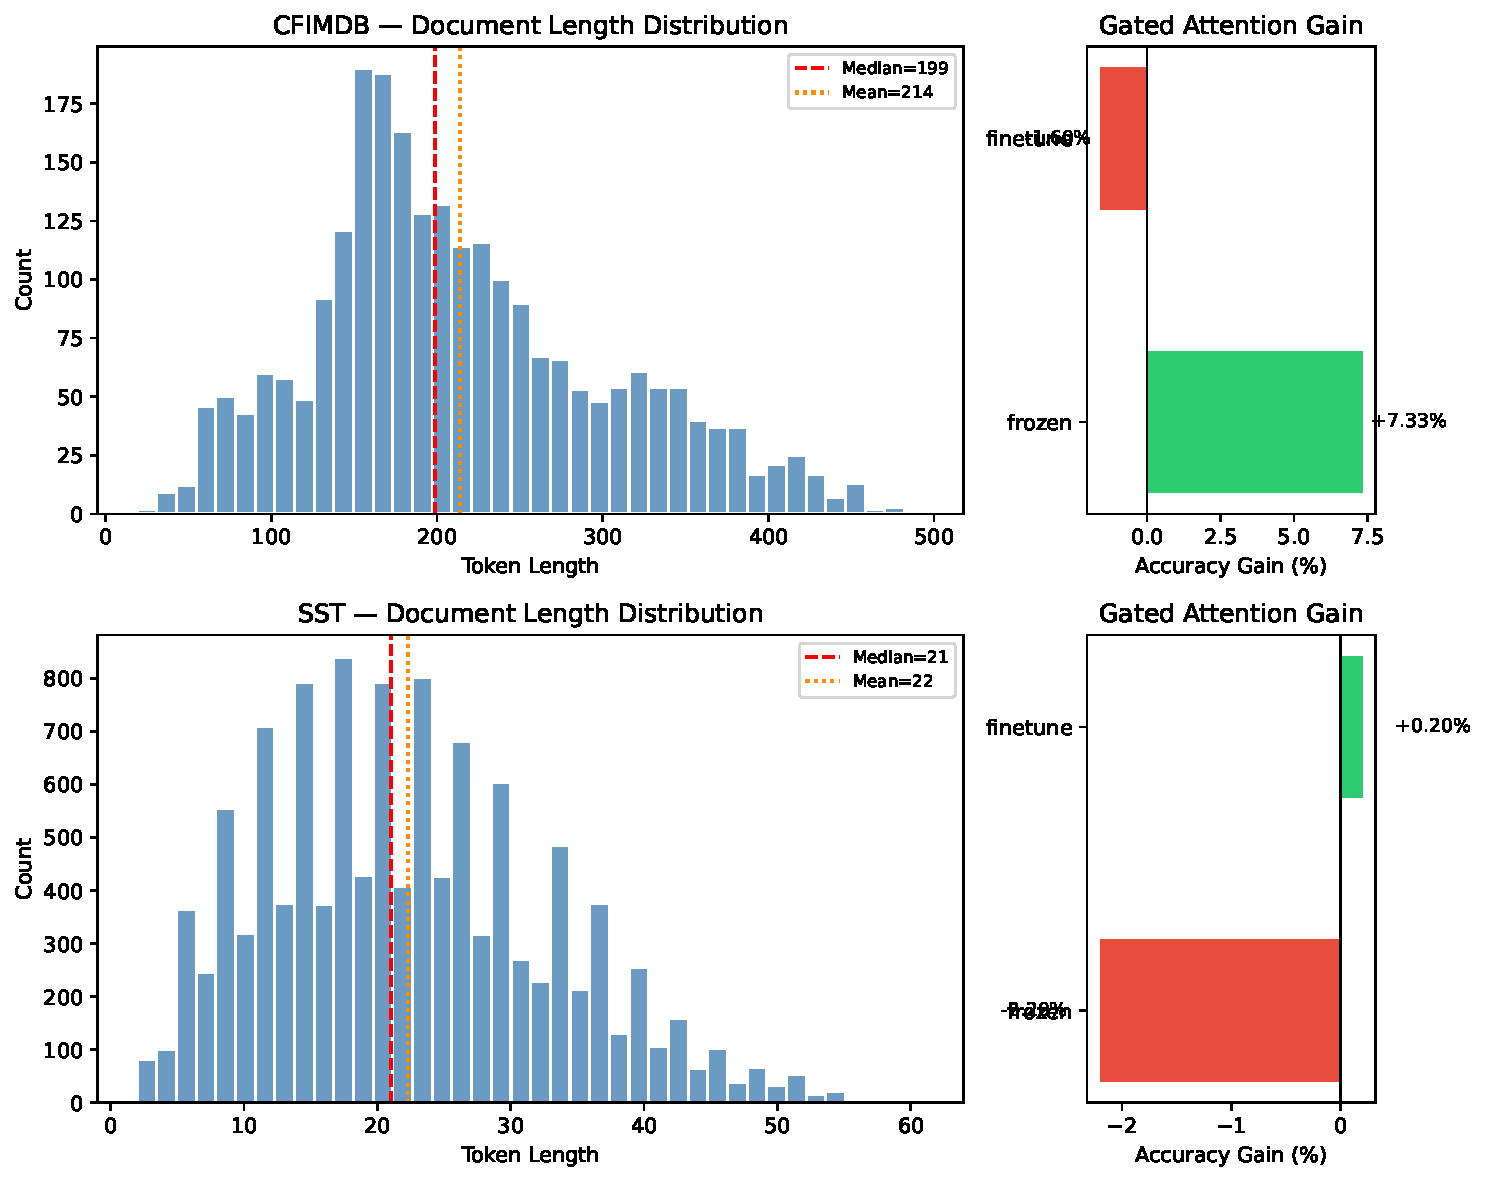
\includegraphics[width=\linewidth]{figures/length_analysis.pdf}
\caption{Left: token length distribution for CFIMDB (top) and SST (bottom). Right: accuracy gain of gated attention vs.\ baseline for each training regime. Gated attention provides the largest benefit on long documents with a frozen encoder.}
\label{fig:length}
\end{figure}

\section{Discussion}

Our results demonstrate that pooling strategy matters significantly for frozen language model encoders. When the backbone LM is frozen---a common scenario in low-resource settings or when model updates are expensive---the classifier head must extract as much information as possible from the fixed representations. Attention pooling provides a simple, parameter-efficient way to do this.

\textbf{Why gated attention outperforms softmax attention.} Standard softmax attention forces scores to sum to one, creating competition: if one sentiment word gets high weight, another must get lower. This is semantically inappropriate for long reviews, where multiple sentiment-bearing phrases (``terrible acting,'' ``waste of time,'' ``poor direction'') should all contribute strongly. Gated attention replaces softmax with independent sigmoid gates, allowing each token to decide its relevance without penalizing other informative tokens. The 1.22\% gain on CFIMDB frozen confirms this: with a frozen encoder, every informative signal must be extracted from the fixed representations, and gating preserves them all rather than forcing them to compete.

\textbf{Why the gap disappears with fine-tuning.} When GPT-2 is fine-tuned, the encoder can reorganize its internal representations to concentrate sentiment information in the final token's hidden state. This makes the pooling strategy less important---the encoder adapts to the task regardless of how the classifier reads out the representation. This observation suggests that for practitioners who can afford full fine-tuning, pooling strategy is a secondary concern. For those operating under computational or parameter constraints that require a frozen encoder, attention pooling offers a meaningful improvement.

\textbf{Limitations.} On short-text datasets like SST, attention pooling does not improve performance. This is consistent with our hypothesis: when the entire input fits comfortably in the causal LM's receptive field, the last token already captures sufficient information. Additionally, both the softmax and gated attention mechanisms use a single head, which cannot capture multiple aspects of sentiment simultaneously---a multi-head variant might provide further benefits. On fine-tuned CFIMDB, gated attention (0.955) underperforms the last-token baseline (0.971), suggesting that when the encoder can adapt, the pooling strategy matters less than the flexibility of the fine-tuned representations. More broadly, fine-tuning a 124M-parameter model on only 1,701 training examples (CFIMDB) leads to overfitting: training accuracy reaches 0.99 while dev accuracy plateaus near 0.96 and later degrades. This is evident across all fine-tuning experiments and is a known challenge when fine-tuning large pre-trained models on small datasets.

\textbf{Broader Implications.} Our approach is general and applicable to any sequence classification task with a frozen encoder. It adds minimal parameters (769 for GPT-2-small) and requires no changes to the underlying model architecture. This makes it particularly useful for deployment scenarios where the encoder must remain fixed (e.g., due to licensing, model size constraints, or multi-task sharing).

\section{Conclusion}

We proposed gated attention pooling as a replacement for both last-token and softmax attention pooling in GPT-2-based sentiment classification. On CFIMDB with a frozen encoder, gated attention improves accuracy from 88.57\% to 95.10\% (+7.33\%), outperforming standard softmax attention (93.88\%) by 1.22\%, with only 769 additional parameters. The key insight is that softmax forces competition between tokens while sigmoid gating allows multiple informative tokens to contribute independently. Our method is simple, lightweight, and general---it can be applied to any sequence classification task with a frozen pre-trained encoder.

\section{Data Availability}

Code and experiment configurations are available at \url{https://github.com/AIU-SoftWave/GPT-2-NLP-Project}. All datasets are publicly available: SST from the Stanford Sentiment Treebank~\citep{socher2013recursive} and CFIMDB from the AIE241 Default Project~\citep{cs224n2024}. Trained model checkpoints and results are included in the supplementary materials.

\section{Acknowledgments}

We thank the AIE241 course staff for providing the project framework, datasets, and reference implementation. We also thank NVIDIA for providing GPU hardware through the academic GPU program.

\section{Funding}

This work was conducted as part of AIE241: Natural Language Processing at AIU.

\section{Conflicts of interest}

The authors declare no conflicts of interest.

\section{Team Contributions}

\textbf{Ahmed Saleh:} Implemented the attention pooling model architecture and training pipeline, conducted experiments on CFIMDB and SST datasets, and led the analysis of attention weight visualizations. \textbf{Mohamed Hany:} Implemented the baseline models and mean pooling ablation, managed the experiment tracking and hyperparameter tuning, and contributed to the training dynamics analysis. \textbf{Mostafa Khamis:} Set up the data processing pipeline, contributed to the literature review on pooling strategies, and assisted with result analysis and report writing.

\bibliography{example-bibliography}

\end{document}
